\section{Introduction}

\begin{frame}{}
  \begin{center}
    {\bf Part I -- Introduction and Motivation}
  \end{center}
\end{frame}

\subsection{Outline}

\begin{frame}{Outline}

  A important point to decide when preparing an experiment is {\bf how
    many observations} are necessary. We call this number the {\bf Sample Size}.\bigskip

  A large sample size can reduce the influence of random noise in the
  calculation of statistical indicators, such as the mean.\bigskip
  
  On the other hand, increasing the sample size also has a cost, in
  time, money or resources.\bigskip

  So how do we choose a proper sample size for an experiment?
\end{frame}

\begin{frame}{Outline}

  In this lecture, we will discuss the following points:\bigskip

  \begin{itemize}
  \item How to think about the sample size;
  \item What factors influence the choice of sample size;
  \item What factors are influenced by the choice of sample size;
  \item How to calculate the desired sample size for certain
    statistical models;
  \end{itemize}

\end{frame}


\subsection{Motivation}

\begin{frame}{Why Repeat an experiment?}{Noise Factors}

  The result of almost any experiment is affected by several
  factors. Some of these factors we can control and understand, {\bf
    but many we cannot}.\bigskip

  {\bf Noise Factors} are these uncontrollable, unknown factors. As
  much as possible, we want to reduce the influence of these factors
  in the result of our experiment.\bigskip

  \alert{{\bf Important:} In most cases, random factors actually have a
    cause, we just don't know it. If you manage to identify the cause
    for some of the random noise, consider if it would be possible to
    remove that noise from your experiment}.
\end{frame}

\begin{frame}{Repeating an experiment to remove noise factors}
  \begin{columns}
    \column{0.2\textwidth}
    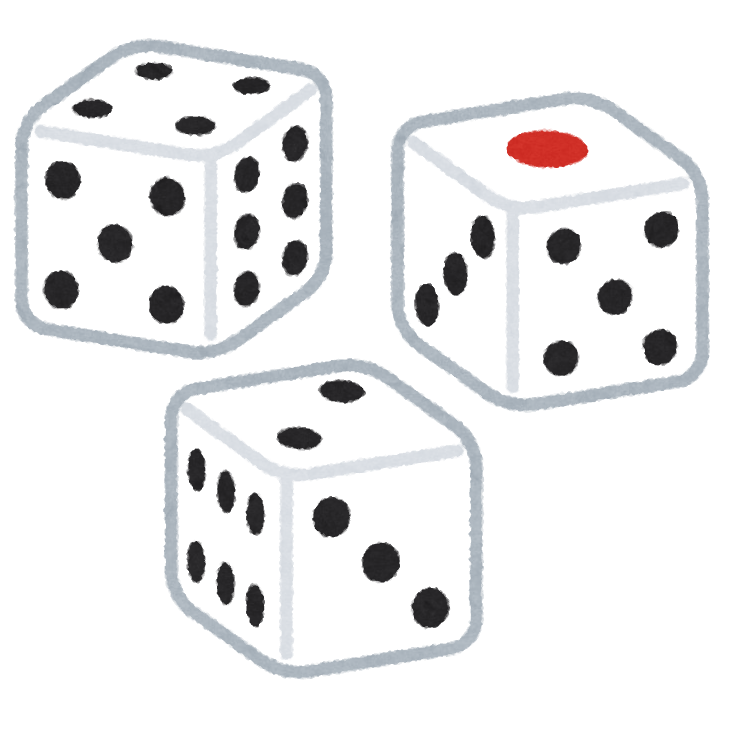
\includegraphics[width=\textwidth]{../img/irasutoya_dice}
    \column{0.8\textwidth} {\bf For example:} When we throw a dice,
    the throw is affected by the air resistance, by small changes in
    our hand movements, by small imperfections in the dice, etc. All
    of these will affect the final result of the dice;
  \end{columns}

  Some assumptions about random noise:
  \begin{itemize}
  \item The variance of random noise is smaller than our minimum interesting difference;
  \item Random noise is unbiased;
  \item Random noise is normally or uniformly distributed;
  \end{itemize}\bigskip

  \begin{block}{}
    You should consider if these assumptions hold true, and maybe
    check them by analyzing the result of a {\bf trial experiment}.
  \end{block}
\end{frame}

\begin{frame}[fragile]{Example: Sample size and Sample Mean Error}

  \begin{columns}
    \column{0.2\textwidth}
      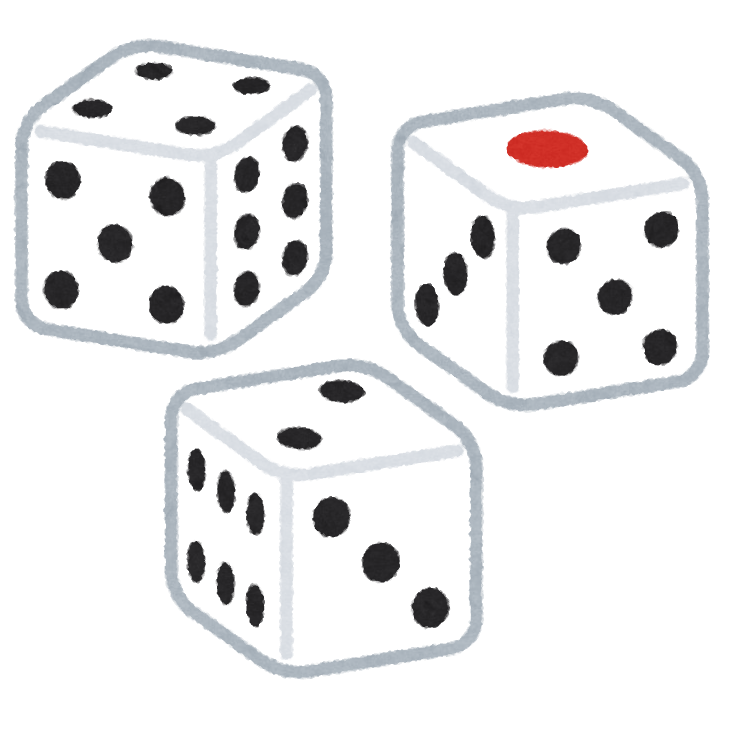
\includegraphics[width=\textwidth]{../img/irasutoya_dice}
      \column{0.8\textwidth}

      Imagine the following simple experiment: We throw three dice,
      and take their sum. We want to estimate the \emph{mean value} of
      this process.\bigskip

      So we repeat the process several times to reduce
      the effect of random noise. What happens when the sample size increase?
    \end{columns}

{\bf The mean and the standard error of the process (10.5 and 2.1), in
  general, will not change much.} However, the standard error of the
{\bf sample mean} will change a lot!
  
{\smaller
\begin{verbatim}
# Three experiments with different sample sizes
sample_2_10 <- replicate(10, mean(replicate(2, sum(sample(6,3)))))
sample_20_10 <- replicate(10, mean(replicate(20, sum(sample(6,3)))))
sample_200_10 <- replicate(10, mean(replicate(200, sum(sample(6,3)))))
# The sample mean is about the same, but the SD of the sample mean changes!
sample size   2: mean of 10 samples: 11.50  sd of 10 samples: 1.90
sample size  20: mean of 10 samples: 10.48  sd of 10 samples: 0.37
sample size 200: mean of 10 samples: 10.56  sd of 10 samples: 0.20 
\end{verbatim}}
\end{frame}

\subsection{Sample Size Considerations}

\begin{frame}{Why should we use large sample sizes?}{}

  Larger sample sizes will reduce (average) the effect of random
  noise, and thus reduce the variance of the indicator.\bigskip

  This will have an effect on:
  \bigskip

  \begin{itemize}
  \item Reduce the size of the confidence interval of the indicator.
  \item Reduce the Type-I error (increase the confidence) of statistical tests.
  \item Reduce the Type-II error (increase the power) of statistical tests.
  \end{itemize}\bigskip
\end{frame}

\begin{frame}{Why should we use SMALL sample sizes?}{}

  Right now, you might be thinking: ``I always want a sample size as big as possible!''\bigskip

  But there are other things to be considered. Experiments usually
  have a {\bf cost} associated with them. Large sample sizes may
  result in large experimental cost:

  \begin{itemize}
  \item Money;
  \item Time;
  \item Resources;
  \item Special conditions;
  \item Ethical considerations;
  \end{itemize}\bigskip

  Also, the increase of sample size has \alert{diminishing returns} in
  terms of reducing experimental error. So we want to use \structure{the
    smallest possible sample size that satisfy our requirements}.
\end{frame}

\begin{frame}{What is a good sample size?}
  For the choice of sample size, we usually take three things in
  consideration:
  \bigskip

  \begin{itemize}
    \item The costs of the experiment; (hard limit to sample size)
    \item The desired \structure{confidence level} (Probability of Type-I error, $\alpha$);
    \item The desired \structure{experimental power} (Probability of Type-II error, $\beta$);
  \end{itemize}\bigskip
\end{frame}

\subsection{Intro to Power Calculation}

\begin{frame}{When you can't choose the sample size, calculate the power}

When an experiment is constrained by budget (not enough time,
not enough money, etc), we might not have a choice of sample size.\bigskip

In this case, {\bf It is important to calculate the confidence and
  power of the experiment}. The power of the experiment will let us
know how reliable the result is.\bigskip

For example, if the power is too low with the available budget, this
information can be used as a justification to require more budget for
the experiment.
\end{frame}


\begin{frame}{Example of Power Calculation}

  To calculate the power of the experiment, we need the following variables:
  \begin{itemize}
  \item Sample size;
  \item Standard deviation;
  \item Significance Level;
  \item Minimum Interesting effect (Delta: $\delta^*$)
  \end{itemize}\bigskip

  The last one is important. $\delta^*$ has a large effect on the
  experiment power. In fact, we usually say something like ``The
  experiment is powerful enough to detect a difference of at least
  $\delta^*$''.
\end{frame}

\begin{frame}[fragile]{Example Calculating the Power with R}

  Let's calculate the power of the dice experiment.\medskip

  Consider a sample size of 20, our observed standard deviation of
  2.1. Can we detect a change in the mean of at least $\delta^*=0.5$,
  with 95\% confidence?

  \smaller{
\begin{verbatim}
> power.t.test(n = 20, sd = 2.1, sig.level = 0.05, 
  + type = "one.sample", alternative = "two.sided", delta = 0.5)

     One-sample t test power calculation 
              n = 20
          delta = 0.5
             sd = 2.1
      sig.level = 0.05
          power = 0.171485                    <-- Very low power
    alternative = two.sided
\end{verbatim}}

It is very likely that our experiment will not detect this difference,
\alert{even if the difference exists!}. Also note that no data was needed!
\end{frame}

\begin{frame}[fragile]{Example Calculating Experiment Power -- changing $\delta^*$}

  Let's repeat the calculation, but change $\delta^*$ to ``1.5''.

  As you can see, the power of the experiment is now $0.85$. This means that the
  experiment with 20 samples is sensitive enough to detect a difference of 1.5 in
  the mean, with 95\% confidence.
  
  \smaller{
\begin{verbatim}
> power.t.test(n = 20, sd = 2.1, sig.level = 0.05, 
  + type = "one.sample", alternative = "two.sided", 
  + delta = 1.5)                              <-- Changing Delta!

     One-sample t test power calculation 
              n = 20
          delta = 0.5
             sd = 2.1
      sig.level = 0.05
          power = 0.85755                     <-- Power increased!
    alternative = two.sided
\end{verbatim}}
\end{frame}

\begin{frame}[fragile]{Example Calculating Experiment Power -- changing the sample size}

  What if we really want to detect a difference of 0.5, with power 0.85?\bigskip

  What is the necessary sample size?
  
  \smaller{
\begin{verbatim}
> power.t.test(power = 0.85,           <-- Fixed power, sample size not given
  + sd = 2.1, sig.level = 0.05, type = "one.sample", 
  + alternative = "two.sided", delta = 0.5)

     One-sample t test power calculation 

              n = 160.311      <-- Necessary Sample Size
          delta = 0.5
             sd = 2.1
      sig.level = 0.05
          power = 0.85
    alternative = two.sided
\end{verbatim}}
\end{frame}

\begin{frame}{Power Calculations: In Summary}{}
  The power calculation can be used to estimate one of the three
  below, \alert{given the other two}:
  \begin{itemize}
  \item The sample size ($n$);
  \item The minimum interesting effect ($\delta^*$)
  \item The experiment power ($\beta$);
  \end{itemize}\bigskip

  Note that for the power calculation, {\bf You don't need the
    data!}\footnote{except for an estimation of the SD}. So
  \structure{It is possible to calculate the sample size before you
    run the experiment}.
\end{frame}

\subsection{The magic number "30"}

\begin{frame}{What about the magic number 30?}{}
  A lot of people have an instinct to use 30 as the ``default'' sample
  size.\bigskip

  This comes from earlier studies that showed that, for many
  distributions, $n = 30$ is enough for the {\bf CLT} to apply, and
  for the {\bf sample mean} to be roughly normally distributed.\bigskip

  This is a very important result! It helps us not worry about the
  assumption of normality. However, other than that, there is nothing
  special about $n=30$\bigskip

  You should always calculate the power of your experiment. Sometimes
  you can use a smaller sample size. Sometimes you need a much bigger sample size.\bigskip

  \alert{Also, it is important to know the power level of your experiment}.  
\end{frame}

\begin{frame}{What about the Variance?}

The Power calculation function is very convenient, but it has a
problem:
\begin{itemize}
\item To calculate the power / sample size, we need to input the standard deviation;
\item To estimate the standard deviation, we need to do an experiment!
\end{itemize}\bigskip

This is a bit of a ``chicken and egg'' problem. There are a few ways to solve this problem:
\begin{itemize}
\item Use knowledge about the problem domain, or historical data, to
  obtain an (initial) estimate;
\item Perform a pilot study to collect a sample only for the SD estimation.
\end{itemize}\bigskip
\end{frame}

\begin{frame}{What about the Variance? -- Pilot Study}{}

  A {\bf Pilot Study} is a small, preliminary experiment. It is used
  to obtain a few estimates about the model under study:
  \begin{itemize}
  \item mean and standard deviation;
  \item possible sources of noise;
  \item possible difficulties in the experiment;
  \end{itemize}

  One way to calculate the pilot study sample size is:
  \begin{equation*}
    n_{\mbox{\textit{pilot}}}\approx 2\left(\frac{z_{\alpha_n/2}}{e_{n}}\right)^2
  \end{equation*}

  \noindent where $(1-\alpha_{n})$ is the desired confidence level for
  the sample size estimate of the main study, and $e_n$ is the maximum
  relative error allowed for the sample size.\bigskip

  This calculation can yield some scarily large sample sizes for a
  pilot study (much larger than would be actually required for the
  main study itself), so use this with caution.
\end{frame}


\section{Specific Sample Size Calculations}
\subsection{}
\begin{frame}{}
  \begin{center}
    {\bf Sample Size Calculations for Specific Models}
  \end{center}
\end{frame}


%%%%%%%%%%%%%%%%%%%%%%%%%%%%%%%%%%%%%%%%%%%%%%%%%%%%%%%%%%
\begin{frame}{Sample Size Calculation for several models}
  Until now, we saw how to calculate the power / sample size for the
  ``1 sample'' model, where we compare one sample against a fixed
  value.\bigskip

  As you may imagine, this calculation will change slighly as the
  statistical model used for the experiment changes. Let's see some of
  these considerations.  
\end{frame}

%   - sample size calculation for post-hoc multi-sample test
%   - Methods for z tests, methods for post-hoc tests
% - Be careful with sample size calculations:
%   - Pseudo-replication (it is not the sample size the matters, but how you choose it.)
%     - An extreme example: We develop an algorithm to solve optimization problems.
%     - The optimization problems have "Types", "Sub-types", and "Sub-Sub types"
%     - We are interested

\subsection{Two Sample Means}

\begin{frame}{Sample size for Two Means}
  Consider the situation where we are comparing the means of two
  samples. For example, the typical experiment where we compare two
  algorithms (A and B) on a single experiment.\bigskip

  While the basic idea is the same, there is a key difference to
  consider here: Should the two sample sizes be the same, or
  different?
\end{frame}


\begin{frame}{Sample Size Calculation}{Example for Two Means}

Consider a case where we are comparing two means with the following
experimental characteristics:\bigskip

\begin{itemize}
  \item Desired significante $\alpha = 0.05$
  \item Desired power: $(1-\beta) = 0.8$;
  \item Minimally relevant effect size (MRES): $\delta^* = 15$
  \item Variances of the samples: $\sigma_1, \sigma_2 = ?$
\end{itemize}\bigskip

What are the required sample sizes for this case?
\end{frame}

\begin{frame}{Sample Size Calculation}{Case 1: Two means, equal variances}

For the specific case of approximately equal variances, {\bf the optimal
sample size ratio is $n_1 = n_2 = n$}, calculated as:

\begin{equation*}
n \approxeq 2\left(\frac{t^{(2n-2)}_{\alpha/2}+t^{(2n-2)}_{\beta}}{d^*}\right)^2
\end{equation*}

where $d^* = \delta^*/\sigma$ is the (standardized) minimally
interesting effect size; and $t^{(2n-2)}_{\alpha/2}$ and
$t^{(2n-2)}_{\beta}$ are the $\alpha/2$ and $\beta$ quantiles of the
$t^{(2n-2 )}$ distribution.\bigskip
\end{frame}

\begin{frame}[fragile]{Sample Size Calculation}{Case 1: Two means, equal variances}

  Let's say that we estimate the standard deviation (for both samples) to be $sd = 15$.\medskip

  We can now calculate the sample size as:
{\smaller
\begin{verbatim}
> ss.calc <- power.t.test(delta = 15,  sd = 15,
                          sig.level = 0.05,  power = 0.8,
                          type = "two.sample",         <-- Two sample model
                          alternative = "one.sided")

  Two-sample t test power calculation
           n = 13.09777             <- NOTE: n is the size of *EACH* sample
       delta = 15
          sd = 15
   sig.level = 0.05
       power = 0.8
 alternative = one.sided
\end{verbatim}}
\end{frame}


\begin{frame}{Sample Size Calculation}{Case 2: Two means, unequal variances}
  When the variance is not the same in both samples, we can use:
  \begin{itemize}
  \item A \structure{balanced} design ($n_1 = n_2$) or;
  \item An \structure{unbalanced} design ($n_1 \neq n_2$)
  \end{itemize}\bigskip

  The unbalanced design usually has a lower total number of
  observations. The optimal allocation of sample size for this kind of
  design is to have the ratio of observations to be equal to the ratio
  of variance:

  $$\frac{n_1}{n_2} = \frac{\sigma_1}{\sigma_2}$$.\bigskip

  (provided that a good estimate of the ratio of variances is available, of course)
  
\end{frame}

\begin{frame}[fragile]{Sample Size Calculation}{Case 2: Two means, unequal variances -- Example unbalanced design}

{\small
\begin{verbatim}
> MESS::power_t_test(n=NULL, sd=15, delta=15, 
+                    ratio=2, sd.ratio=2,
+                    power=0.8, sig.level = 0.05,
+                    type="two.sample", alternative="one.sided")

Two-sample t test power calc with unequal sample sizes and unequal variances 

              n = 19.01525, 38.03050 <-- bigger sample size
          delta = 15
             sd = 15, 30             <-- total var is lager
      sig.level = 0.05
          power = 0.8
    alternative = one.sided

NOTE: n is vector of number in each group
\end{verbatim}}
\end{frame}

\begin{frame}[fragile]{Sample Size Calculation}{Case 2: Two means, unequal variances -- Example balanced design}

{\small
\begin{verbatim}
> MESS::power_t_test(n=NULL, sd=15, delta=15, 
+                    ratio=1, sd.ratio=2,
+                    power=0.8, sig.level = 0.05,
+                    type="two.sample", alternative="one.sided")
     Two-sample t test power calculation with unequal variances 

              n = 31.8629, 31.8629 <-- larger total observations
          delta = 15
             sd = 15, 30
      sig.level = 0.05
          power = 0.8
    alternative = one.sided

NOTE: n is number in *each* group
\end{verbatim}}
\end{frame}

\begin{frame}[fragile]{Sample Size Calculation}{Case 2: Two means, unequal variances -- Example power calculation}

{\small
\begin{verbatim}
> MESS::power_t_test(n=20, sd=15, delta=15, 
+                    ratio=1.5, sd.ratio=2,
+                    power=NULL, sig.level = 0.05,
+                    type="two.sample", alternative="one.sided")

Two-sample t test power calc with unequal sample sizes and unequal variances 

              n = 20, 30
          delta = 15
             sd = 15, 30
      sig.level = 0.05
          power = 0.7438965 <-- lower power
    alternative = one.sided

NOTE: n is vector of number in each group
\end{verbatim}}
\end{frame}


\begin{frame}{Sample Size Calculation}{Two means, unequal variances considerations}

  \begin{itemize}
  \item We can use a balanced design, but the total number of observations will be higher.
  \item Using an unbalanced design will result in a smaller total sample size.
  \item We should calculate the power if the sample size is fixed.
  \end{itemize}

\end{frame}

%%%%%%%%%%%%%%%%%%%%%%%%%%%%%%%%%%%%%%%%%%%%%

\begin{frame}{Comparison of two means -- Paired design}{}


  The analysis of an experiment with \structure{paired design} can
  require smaller sample sizes for the same power.\bigskip

  This happens when the {\bf between-units variation~($\sigma_U$)} is relatively
  high, and the {\bf in-unit variation ($\sigma_\epsilon$)} is relatively
  homogeneous.\bigskip

  For large enough $n$~(e.g., $n\geq 10$), we have that:

\begin{equation*}
\frac{n_{\mbox{\tiny unpaired}}}{n_{\mbox{\tiny paired}}}\approx\sqrt{2\left[\left(\frac{\sigma_u}{\sigma_\epsilon}\right)^2+1\right]}
\end{equation*}

  So we can initially calculate the unpaired sample size, and adjust it for the paired case.
\end{frame}

\begin{frame}[fragile]{Comparison of two means -- Paired design}{}
  Alternatively, we can also use good old \emph{power\_t\_test}:

{\small
\begin{verbatim}
> MESS::power_t_test(n=NULL, sd=15, delta=15, 
+                    ratio=1, sd.ratio=1,
+                    power=0.8, sig.level = 0.05,
+                    type="paired", alternative="one.sided")

     Paired t test power calculation 

              n = 7.727622       <-- paired tests are very powerful!
          delta = 15
             sd = 15             <-- don't forget you have to show this!
      sig.level = 0.05
          power = 0.8
    alternative = one.sided

NOTE: n is number of *pairs*, sd is std.dev. of *differences* within pairs
\end{verbatim}
}
\end{frame}


% % Equivalence testing
% \begin{frame}{Sample size for Equivalence of a single mean}
% Sample sizes for testing equivalence of a single mean can be derived using essentially the same considerations used for the usual tests. In the case of a single sample:
%
% \begin{equation*}
% n\geq\left(\frac{\left(t_{\alpha}+t_{\beta}\right)\hat{\sigma}}{\delta^* - \Delta\mu}\right)^2
% \end{equation*}
% \bigskip
%
% As in the previous cases, iteration is needed to solve for $n$ (since the quantiles of the t distribution depend on $n$). Use $t_x$ = $z_x$ for the first iteration.
% \end{frame}
%
% \begin{frame}
% {Sample size for Equivalence of two means}
%
% Sample size for the $n_1 = n_2 = n$ case can be approximated based on the Zhang formula.
% $$n \geq \left(t_{\alpha;\nu}+t_{(1-c)\beta;\nu}\right)^2\left(\frac{\hat{\sigma}_1^2+\hat{\sigma}_2^2}{\delta^*-\Delta\mu^*}\right)^2$$
%
% \noindent with $\Delta\mu^*<\delta^*$ as the maximum real difference between the two means for which a power of $(1-\beta)$ is desired, and:
% $$c = \frac{1}{2}\exp\left(-7.06\frac{\Delta\mu^*}{\delta^*}\right)$$
% \end{frame}

\subsection{Sample Size for ANOVA}

\begin{frame}{Sample Size Calculation for multiple means}

  The analysis of multiple means, as discussed in a previous class, is composed of two steps:
  \begin{itemize}
  \item Overall analysis using ANOVA;
  \item Posthoc analysis between pairs of samples;
  \end{itemize}\bigskip

  So when calculating sample size, we can use the calculation for the
  first part, or for the second part. Usually the second part implies
  a larger sample size, but sometimes we want to know the power for
  the first part too.  
\end{frame}

\begin{frame}{Power calculation for the ANOVA}{Scenarios of Interest}
  The power of a test is the probability of the test not being able to
  detect the alternate hypothesis (type II error). So to calculate the
  power of ANOVA, we need to establish a {\bf scenario of interest}.\medskip 

  For example, if we are comparing 4 samples, two scenarios tend to be
  of interest:\bigskip

\noident The first is if we have two levels biased symmetrically about the
  grand mean, and all the others equal to zero:

$$ \tau = \left\{-\frac{\delta^*}{2}, \frac{\delta^*}{2}, 0, 0\right\}$$

\noindent and the second is if we have one level biased in relation to
all others:

$$ \tau = \left\{-\frac{(a-1)\delta^*}{a}, \frac{\delta^*}{a}, \frac{\delta^*}{a}, \frac{\delta^*}{a}\right\}$$
\end{frame}

\begin{frame}{Power calculation for the ANOVA}{General Formula}
  
Given the scenario of interest, the power/sample size calculations
boil down to the equality:

\begin{equation*}
F_{(1-\alpha)} = F_{\beta;\phi}
\end{equation*}

with both $F$ distributions having $(a-1)$ degrees of freedom in the
numerator and $a(n-1)$ in the denominator. The noncentrality parameter
$\phi$ is given by:

\begin{equation*}
\phi = \frac{n\sum\limits_{i=1}^{a}\tau_i^2}{\hat{\sigma}^2}
\end{equation*}
\end{frame}

\begin{frame}[fragile]{Power calculation for the ANOVA}{Example}

To ilustrate, imagine an experimental design with $a = 4,\ \alpha =
0.05,\ \hat{\sigma} = 7$, and suppose that the researcher wants to be
able to detect whether any two means present differences of magnitude
$\delta^* = 12$ with power $(1-\beta)=0.8$.\bigskip

For the first scenario of interest we have a noncentrality parameter of:

$$\phi = \frac{4\left(6^2+6^2+0+0\right)}{7^2} = 5.88$$
\end{frame}

\begin{frame}[fragile]{Power calculation for the ANOVA}{Example}
And we can calculate the power/sample size of the first scenaro as:

{\smaller
\begin{verbatim}
> a       <- 4                         > alpha   <- 0.05
> sigma   <- 7                         > delta   <- 12
> beta    <- 0.2
> tau <- c(-delta/2, delta/2, 0, 0)
> vartau <- var(tau)

> power.anova.test(groups = 4, between.var = vartau,
+                  within.var = sigma^2, sig.level = alpha,
+                  power = 1 - beta)$n
[1] 8.463358
\end{verbatim}}
\end{frame}

%=====


\begin{frame}[fragile]{Power calculation for the ANOVA}{Example}
The second case (one level biased in relation to all others) is also quite easy to calculate:

{\smaller
\begin{verbatim}
> tau <- c(-delta*(a - 1)/a, rep(delta/a, a - 1))
> vartau <- var(tau)
> power.anova.test(groups = 4, between.var = vartau,
+                  within.var = sigma^2, sig.level = alpha,
+                  power = 1 - beta)$n
[1] 6.018937
\end{verbatim}}

It is important to remember that these are the sample sizes required
for the ANOVA only - any multiple comparisons procedure executed
afterwards to pinpoint the significant differences will have smaller
power for same-sized effects (unless more observations are
added). This is one reason why it is common to design experiments
calculating the sample sizes based on the multiple comparisons
procedure, instead of using the ANOVA formulas.
\end{frame}

\subsection{}
\begin{frame}{More on sample size calculation for Computer Science experiments}

  These formulas and concepts only scratch the surface of the problem of sample size calculation. \bigskip

  By understanding the characteristics of the populations under study, we can identify a minimum sample size that gives us a test with desired confidence and power.\bigskip

  A more recent discussion of the calculation of sample sizes for the specific case of algorithm comparison is the paper by Felipe Campelo:\\
  \url{https://link.springer.com/article/10.1007/s10732-018-9396-7}\bigskip

  I highly recommend reading this paper as a complement to this lecture.
\end{frame}

\begin{frame}{Recommended Reads}
  \begin{itemize}
    \item Felipe Campelo \emph{"Sample size estimation for power and accuracy in the experimental comparison of algorithms"}, 2019
    \url{https://link.springer.com/article/10.1007/s10732-018-9396-7}
    \item Paul Mathews' \textit{Sample Size Calculations}, MMB, 2010.
    \item Zhang (2003), J. Biopharm. Stat. 13(3):529-538.
  \end{itemize}
\end{frame}
